% !TEX program = xelatex
% !TEX output_directory = .
\documentclass[12pt,a4paper,fontset=fandol]{ctexart}

\usepackage[margin=1in]{geometry}
\usepackage{amsmath}
\usepackage{amssymb}
\usepackage{booktabs}
\usepackage{multirow}
\usepackage{graphicx}
\usepackage{subcaption}
\usepackage{float}
\usepackage{hyperref}
\usepackage{longtable}
\usepackage{array}
\usepackage{xcolor}
\usepackage{grffile}

\hypersetup{
  colorlinks=true,
  linkcolor=blue,
  urlcolor=blue,
  citecolor=blue
}

\graphicspath{
  {../project_outputs/part_b/}
  {../project_outputs/part_c/}
  {../project_outputs/part_c_extended_drop_last/}
  {project_outputs/part_b/}
  {project_outputs/part_c/}
  {project_outputs/part_c_extended_drop_last/}
}

\title{Neural Network and Deep Learning Project 1\\
\large MNIST 上的 MLP、CNN 与鲁棒性引导增强研究}
\author{
姓名：\underline{黄德超}\\
学号：\underline{23300660009}
}
\date{\today}
\setlength{\emergencystretch}{2em}

\begin{document}

\maketitle

\noindent
\textbf{Github 链接：}
\href{https://github.com/adehuang41/deep_learning_pj1.git}
{\texttt{https://github.com/adehuang41/deep\_learning\_pj1.git}}

\noindent
\textbf{模型权重 / Checkpoint 链接：}
\href{https://your-checkpoint-link}{\texttt{待上传后补充真实链接}}

\begin{abstract}
本报告围绕 MNIST 手写数字分类，完成了课程项目要求的三个实验模块。Part A 建立了从零实现的 MLP baseline；Part B 在统一训练协议下比较了 MLP 与 CNN；Part C 选择 \texttt{Data Augmentation} 和 \texttt{Robustness Analysis} 两个方向，并将它们组织成一个统一问题：先诊断 \texttt{CNN-clean} 的主要脆弱扰动，再比较从头增强训练与基于已有 clean CNN 的 targeted fine-tuning。结果表明：CNN 在 clean MNIST 上明显优于 MLP，且参数量更少；在 Part C 中，验证集诊断选出的主要弱点是 \texttt{translation-3}，针对该扰动训练可以显著提升鲁棒性，其中 \texttt{CNN-AugScratch-target} 效果最强，而 \texttt{CNN-RGFT-target} 在较低边际成本下也取得了很强的修复效果。进一步的 extension 结果表明，简单地只选择最脆弱的 hard subset 并不一定优于随机子集，这一 negative finding 说明鲁棒性诊断适合暴露失败样本，但低成本修复仍然依赖足够的数据分布覆盖。
\end{abstract}

\section{Introduction and Experimental Setup}

本项目按实验流程组织报告，而不是机械地把课程说明中的六项要求拆成六个并列一级标题。具体来说，\texttt{MLP baseline}、\texttt{CNN comparison} 和 \texttt{two additional directions} 构成实验主线；\texttt{main results table}、\texttt{detailed visualization} 和 \texttt{discussion} 被整合进对应实验部分，并在最后集中总结。因此，本报告覆盖了老师要求的全部内容，但采用了更自然的 experimental-flow 结构。

数据集为标准 MNIST。原始训练集共有 60{,}000 张图像，我使用固定随机种子 309 将其划分为 50{,}000 张训练图像和 10{,}000 张验证图像。验证集用于 checkpoint 选择、鲁棒性诊断和 target 选择；官方 10{,}000 张测试集在最终评估之前保持不参与训练和模型选择。除训练随机性之外，鲁棒性评估还固定使用单独的评估随机种子 2026，以保证不同模型之间的 perturbation 采样一致。

所有模型都使用归一化到 $[0,1]$ 的灰度输入。Part A 和 Part B 采用相同的 train/validation split、相同预处理、相同优化器类型和相同 epoch budget；Part C 在此基础上保持同一 clean baseline，再做 target-aware augmentation 或 fine-tuning。主要训练设置见表 \ref{tab:setup}.

\begin{table}[H]
  \centering
  \small
  \caption{Main training settings used in this project.}
  \label{tab:setup}
  \renewcommand{\arraystretch}{1.08}
  \begin{tabular}{lccc}
    \toprule
    Experiment & Epochs & Batch size & Learning rate \\
    \midrule
    \texttt{MLP-clean} & 30 & 256 & 0.05 \\
    \texttt{CNN-clean} & 30 & 256 & 0.01 \\
    \texttt{CNN-AugScratch-target} & 30 & 64 & 0.01 \\
    \texttt{CNN-RGFT-target} & 10 & 64 & 0.005 \\
    RGFT extension variants & 10 & 64 & 0.005 \\
    \bottomrule
  \end{tabular}
\end{table}

关于 \texttt{translation-3} 的实现需要明确说明。训练阶段的 target augmentation 采用 online random translation：对每张图像在横纵两个方向分别随机采样整数位移，范围均为 $[-3, 3]$，超出边界的部分裁剪，新暴露区域用零填充。主线 validation/test 评估中的 \texttt{translation-3} 也沿用这一实现，但使用固定评估随机种子，因此比较是可复现的。与之不同，extension 中 hard subset 的构造采用四个确定方向的 \texttt{left/right/up/down} 平移评分，这个 deterministic four-direction scoring 仅用于 subset selection，而不是主线 Part C 的总体测试指标。

\section{MLP Baseline}

Part A 的目标是建立一个可运行、可解释的 MLP baseline，并验证线性层和 softmax cross-entropy 的前向与反向传播实现正确。模型采用单隐层结构 $784 \rightarrow 256 \rightarrow 10$，激活函数为 ReLU，训练使用 SGD。

\texttt{MLP-clean} 的最终结果如下：
\begin{itemize}
  \item 训练准确率：0.9698
  \item 验证准确率：0.9601
  \item 测试准确率：0.9640
\end{itemize}

这个结果说明 Part A 的基础训练链路已经工作正常，同时为后续 MLP-vs-CNN 比较提供了一个足够强的 clean baseline，而不是一个明显欠拟合的对手。

\begin{figure}[H]
  \centering
  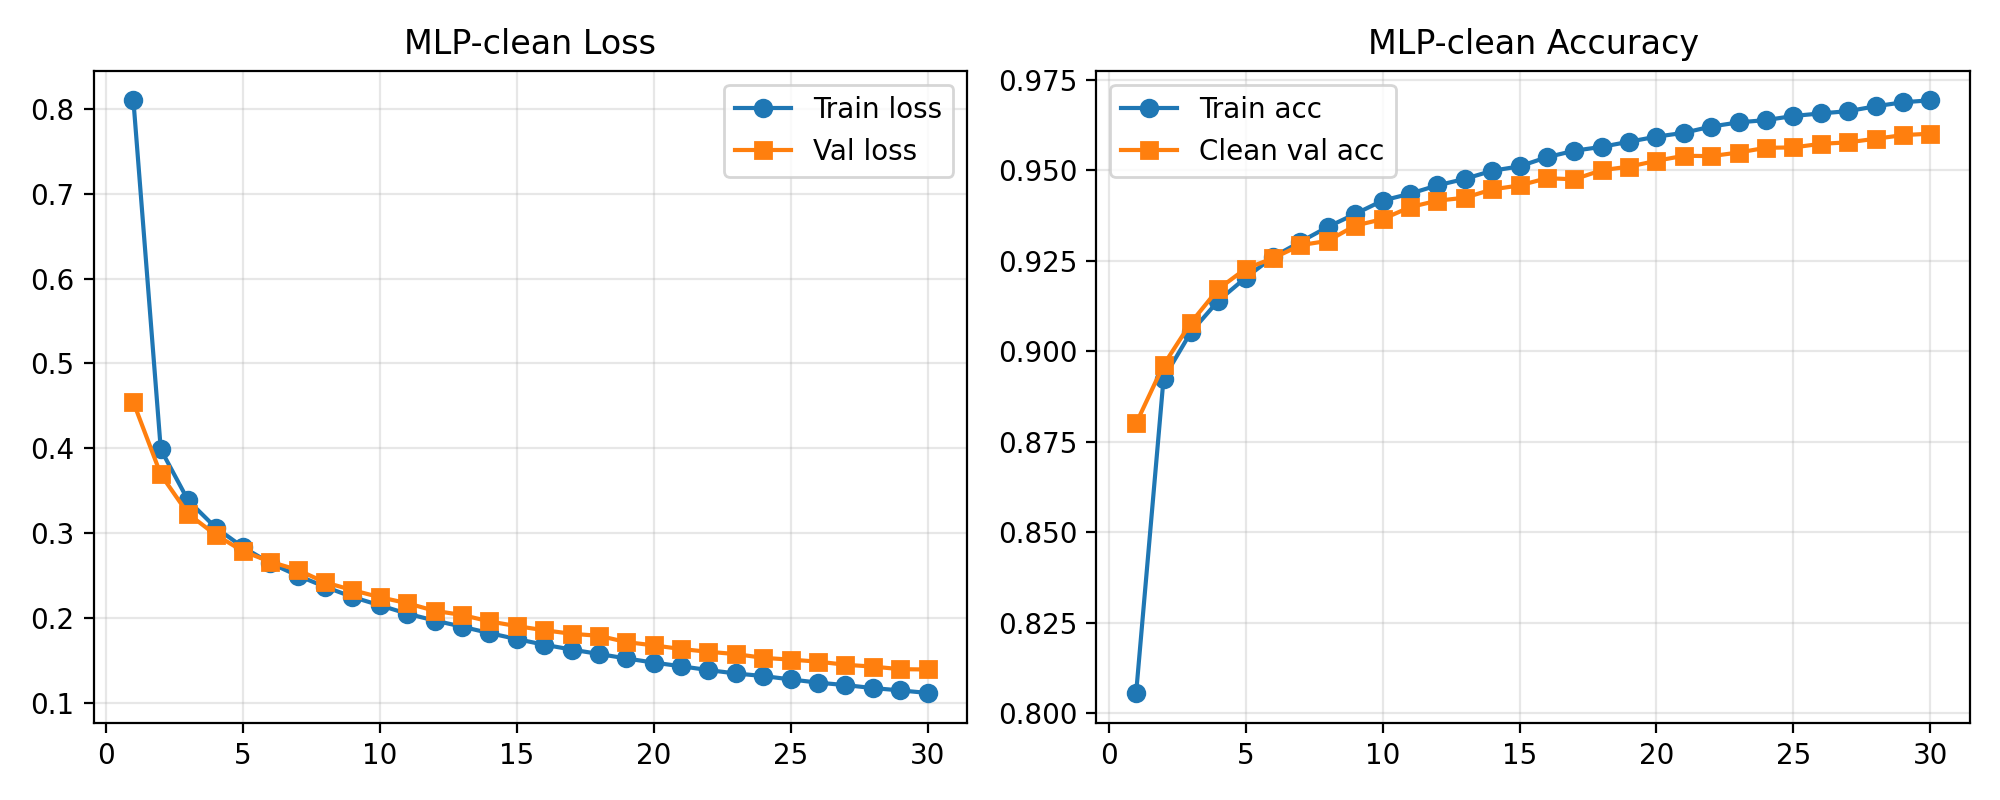
\includegraphics[width=0.72\textwidth]{mlp_learning_curve.png}
  \caption{\texttt{MLP-clean} 的训练曲线。}
\end{figure}

\section{CNN Model and MLP-vs-CNN Comparison}

\subsection{Model architecture and fair comparison protocol}

Part B 中，我实现了一个教学型小 CNN。为避免横向公式超页，结构按层展开如下：

\begin{center}
\begin{tabular}{ll}
Input & $1 \times 28 \times 28$ \\
Conv1 & $1 \to 8$, kernel $3 \times 3$, padding $=1$ \\
ReLU + MaxPool & $2 \times 2$ \\
Conv2 & $8 \to 16$, kernel $3 \times 3$, padding $=1$ \\
ReLU + MaxPool & $2 \times 2$ \\
Flatten & $16 \times 7 \times 7 = 784$ \\
FC1 & $784 \to 128$ \\
ReLU & -- \\
FC2 & $128 \to 10$ \\
\end{tabular}
\end{center}

卷积、池化、全连接和交叉熵损失都使用本项目中的 NumPy 实现，没有调用 PyTorch、TensorFlow 或 JAX 的同类深度学习模块。为了保证 MLP 与 CNN 的比较尽量公平，我保持了相同的 train/validation split、相同的数据预处理、相同的 batch size（256）、相同的 epoch budget（30）以及相同的优化器类型（SGD）。学习率只做最小必要调整：MLP 使用 0.05，CNN 使用 0.01，以保证两种结构都能稳定训练。

\subsection{Main results of Part B}

\begin{table}[H]
  \centering
  \caption{Part B 中 \texttt{MLP-clean} 与 \texttt{CNN-clean} 的主要结果。}
  \begin{tabular}{lcccc}
    \toprule
    模型 & 参数量 & Train Acc & Val Acc & Test Acc \\
    \midrule
    \texttt{MLP-clean} & 203530 & 0.9698 & 0.9601 & 0.9640 \\
    \texttt{CNN-clean} & 103018 & 0.9823 & 0.9757 & 0.9799 \\
    \bottomrule
  \end{tabular}
\end{table}

\texttt{CNN-clean} 在验证集和测试集上都明显优于 \texttt{MLP-clean}，测试准确率提升约 1.59 个百分点。同时，CNN 的可训练参数量只有 103018，约为 MLP 的一半。这说明它的优势并不来自更大的模型规模，而是来自更适合图像任务的结构偏置。

\begin{figure}[H]
  \centering
  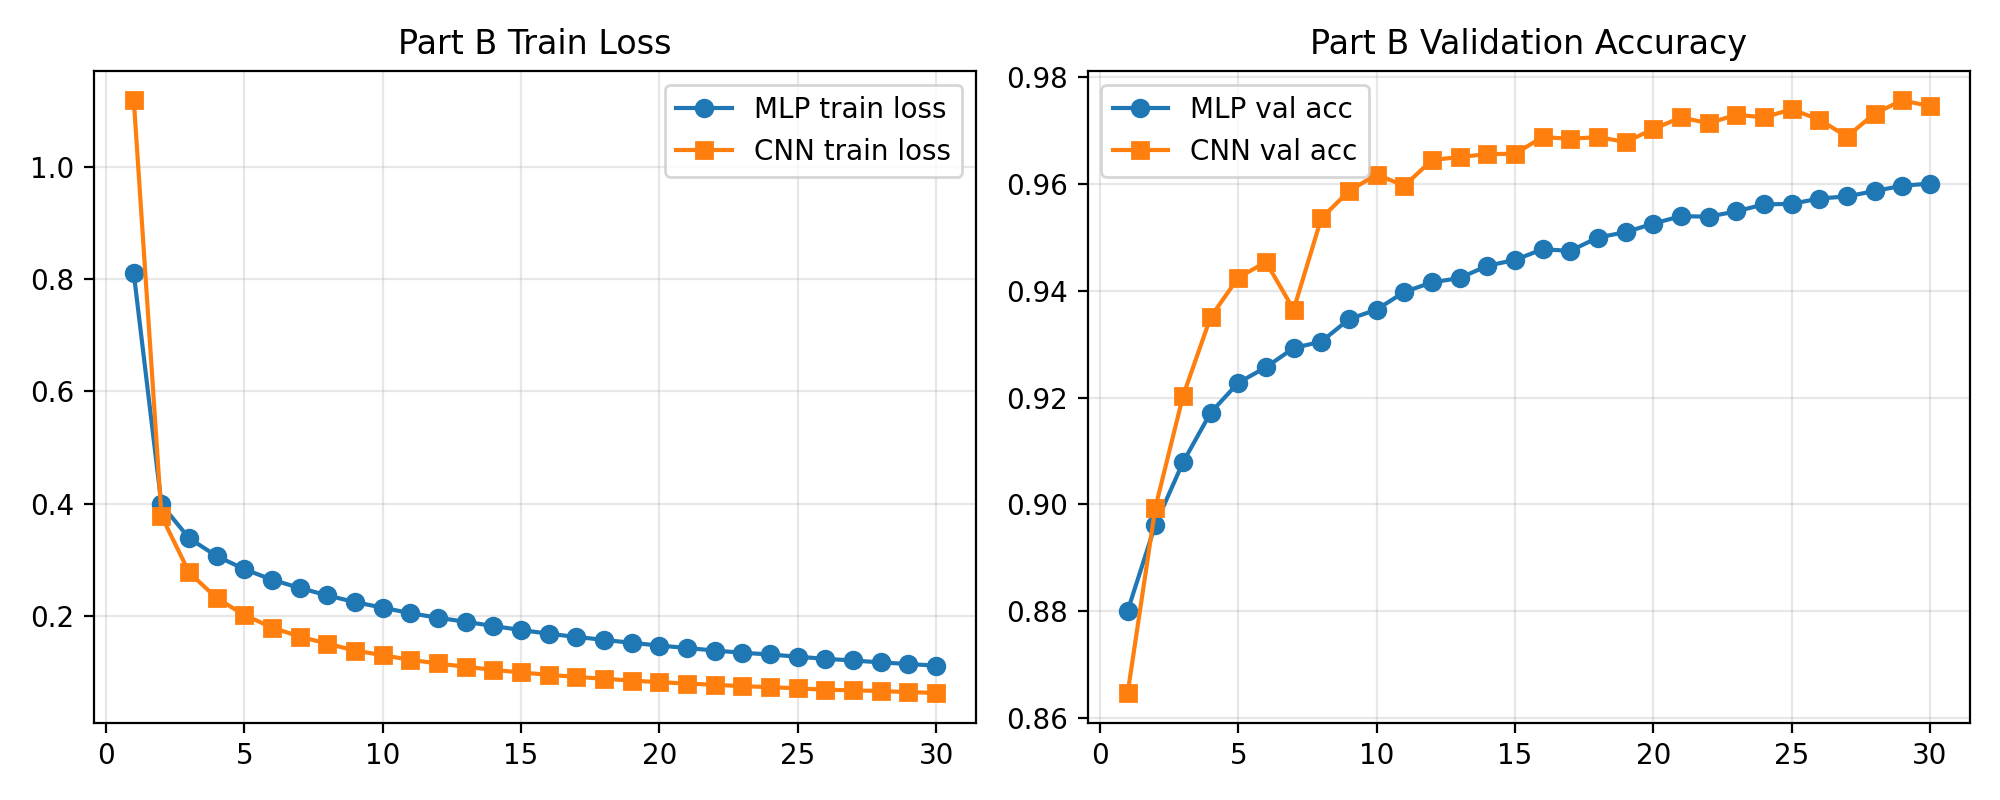
\includegraphics[width=0.78\textwidth]{mlp_vs_cnn_learning_curve.png}
  \caption{\texttt{MLP-clean} 与 \texttt{CNN-clean} 的对比训练曲线。}
\end{figure}

\begin{figure}[H]
  \centering
  \begin{subfigure}{0.48\textwidth}
    \centering
    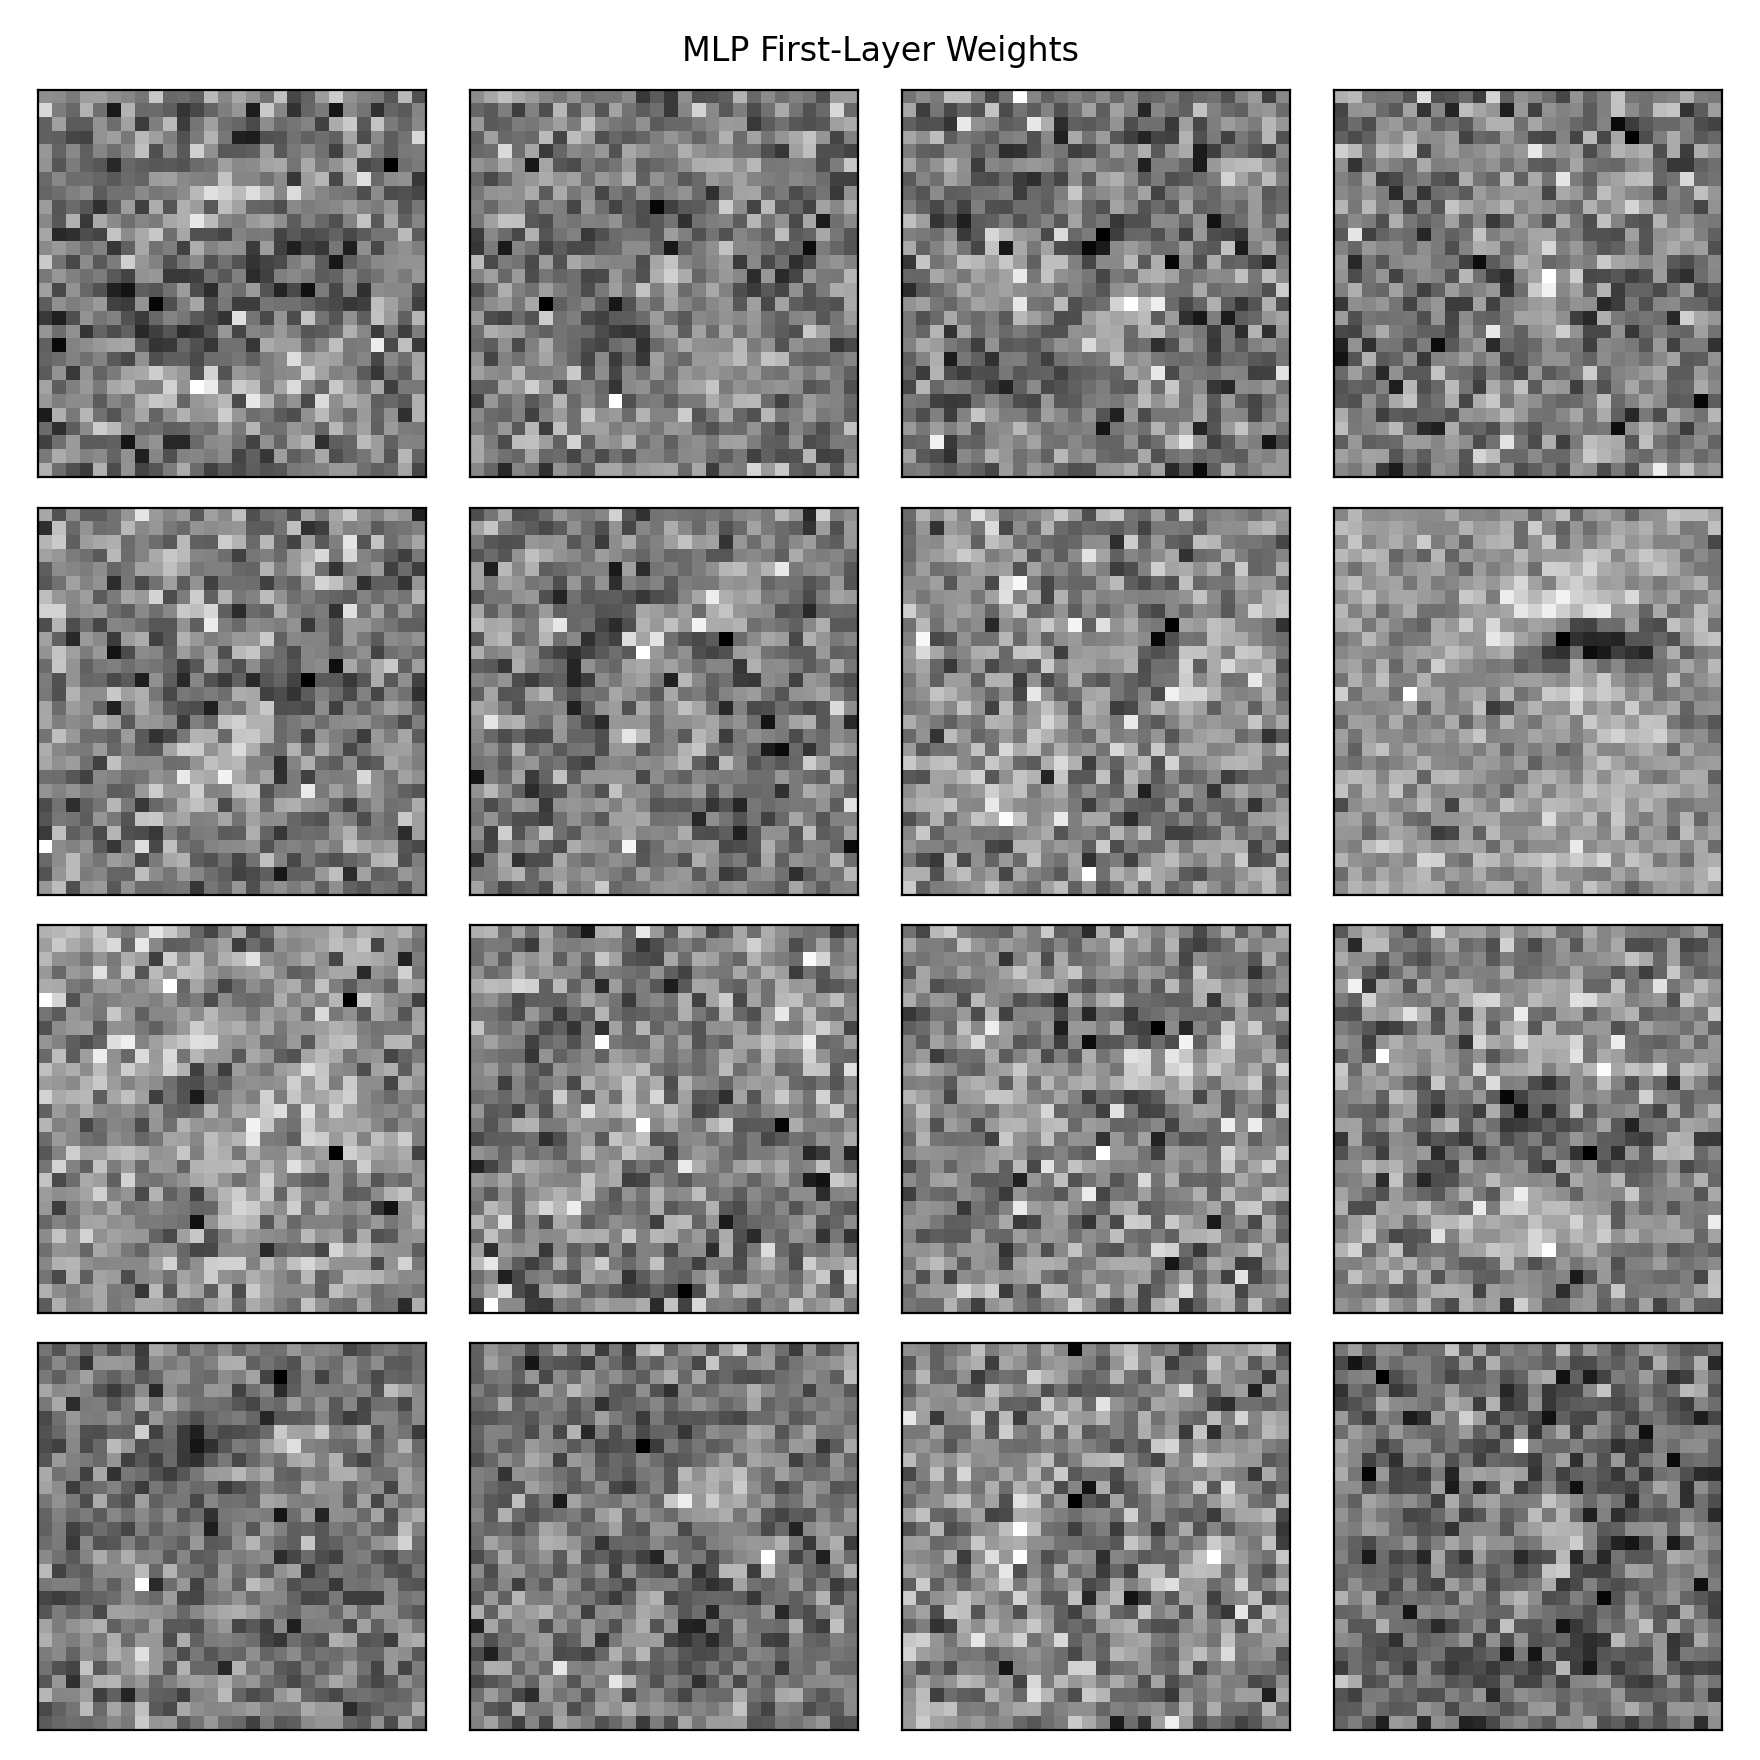
\includegraphics[width=\textwidth]{mlp_first_layer_weights.png}
    \caption{MLP 第一层权重可视化}
  \end{subfigure}
  \hfill
  \begin{subfigure}{0.48\textwidth}
    \centering
    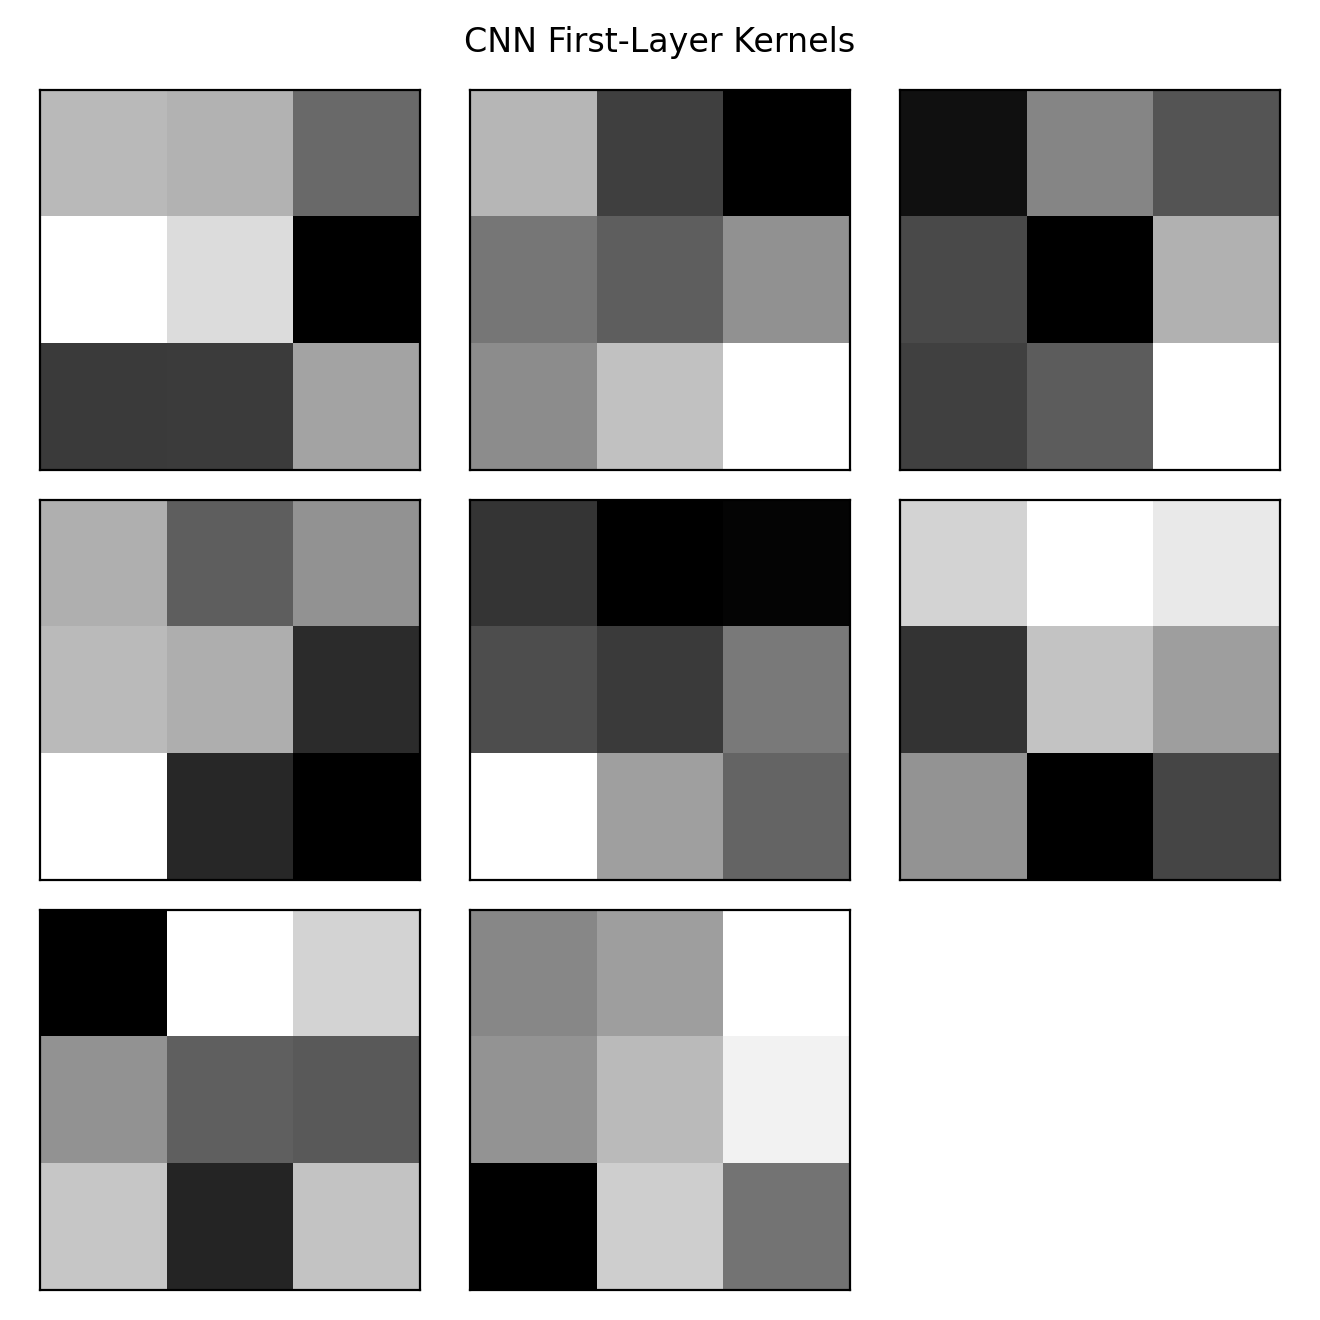
\includegraphics[width=\textwidth]{cnn_first_layer_kernels.png}
    \caption{CNN 第一层卷积核可视化}
  \end{subfigure}
  \caption{Part B 的解释性可视化。}
\end{figure}

\subsection{Why the CNN is better suited to image classification}

本实验结果支持以下结构性解释。第一，MLP 在输入层前就把 $28 \times 28$ 图像 flatten 成长度为 784 的向量，显式二维空间邻域被打散。第二，CNN 的 local receptive field 更契合手写数字由局部笔画构成的特点。第三，weight sharing 带来了更高的参数效率，因此相同模式出现在不同位置时不需要重复学习。第四，卷积是 translation-equivariant，而 pooling 和后续空间聚合会提高模型对小范围位移的容忍度。第五，多层卷积可以把低级边缘和笔画段逐步组合成更完整的数字部件。

需要保持表述严谨：普通 CNN 并不会自动获得完美的 translation invariance，更不会天然具有 rotation invariance。事实上，Part C 之所以最终选择 \texttt{translation-3} 作为 target perturbation，正是因为它在验证集上给 \texttt{CNN-clean} 造成了最大的 accuracy drop。这说明 CNN 虽然比 MLP 更适合图像局部模式，但对更强的空间位移仍然存在明确弱点。

\section{Robustness-Guided Data Augmentation}

\subsection{Robustness diagnosis and target selection}

Part C 选择了两个 additional directions：
\begin{itemize}
  \item Direction 3: \texttt{Data Augmentation}
  \item Direction 4: \texttt{Robustness Analysis}
\end{itemize}

这两个方向没有被拆成两个彼此独立的小实验，而是被组织成同一个研究问题：先通过 validation robustness diagnosis 找到 \texttt{CNN-clean} 的主要弱点，再围绕该弱点比较两种 target-aware 训练策略。

我先在验证集上评估 \texttt{CNN-clean} 在以下扰动下的表现：
\begin{itemize}
  \item Gaussian noise: $\sigma = 0.05, 0.10, 0.20$
  \item translation: severity $= 1, 2, 3$
  \item rotation: angle $= 5^\circ, 10^\circ, 15^\circ$
\end{itemize}

target perturbation 的选择规则很简单：只看 overall validation accuracy drop，选取掉点最大的单一设置。最终选出的 target 为 \texttt{translation-3}。因此，后续所有 target-aware 训练和目标指标都围绕这一具体设置展开，而不是笼统地说“提升了平移鲁棒性”。

\begin{figure}[H]
  \centering
  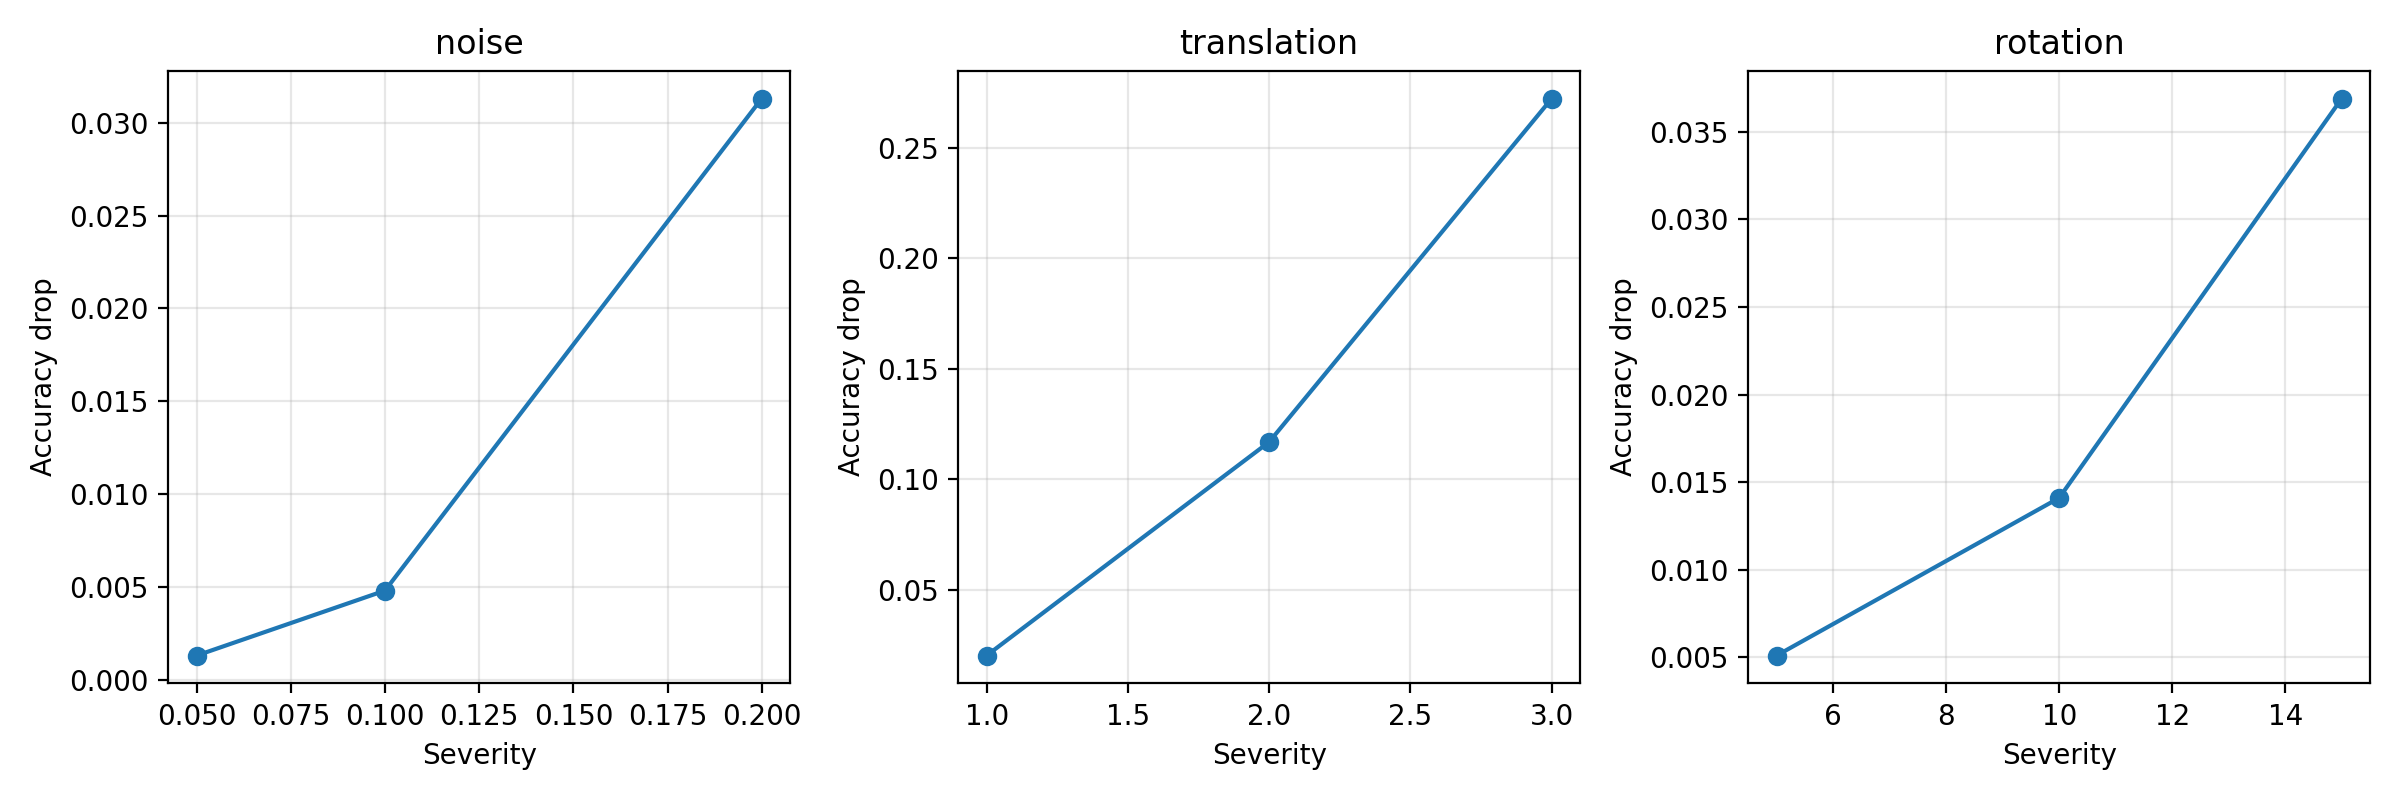
\includegraphics[width=0.80\textwidth]{validation_robustness_curve.png}
  \caption{Validation robustness diagnosis for \texttt{CNN-clean}.}
\end{figure}

\subsection{AugScratch vs full-data RGFT}

在选定 \texttt{translation-3} 之后，我比较了两种训练策略。

\paragraph{\texttt{CNN-AugScratch-target}}
从头训练一个新的 CNN，训练时每个 mini-batch 由 50\% clean 样本和 50\% target-perturbed 样本组成，epoch budget 为 30。

\paragraph{\texttt{CNN-RGFT-target}}
从 \texttt{CNN-clean} 的 best checkpoint 出发，继续做 targeted fine-tuning。训练同样采用 50\% clean samples and 50\% target-perturbed samples，但只追加 10 个 fine-tuning epochs。checkpoint selection 遵循一个显式约束：在 clean validation accuracy 相比 \texttt{CNN-clean} 下降不超过 1 个百分点的前提下，选择 target validation accuracy 最高的 checkpoint。

\begin{table}[H]
  \centering
  \small
  \caption{Part C 主线结果。}
  \renewcommand{\arraystretch}{1.08}
  \begin{tabular}{lccccc}
    \toprule
    模型 & Clean & Target & Target Drop & Neighbor & 说明 \\
    \midrule
    \texttt{MLP-clean} & 0.9640 & 0.5320 & 0.4320 & 0.7248 & 参考基线 \\
    \texttt{CNN-clean} & 0.9799 & 0.7069 & 0.2730 & 0.8654 & clean CNN \\
    \texttt{CNN-AugScratch-target} & 0.9815 & 0.9568 & 0.0247 & 0.9728 & 从头增强训练 \\
    \texttt{CNN-RGFT-target} & 0.9790 & 0.9266 & 0.0524 & 0.9590 & targeted fine-tuning \\
    \bottomrule
  \end{tabular}
\end{table}

结果非常清楚。第一，即使在增强之前，\texttt{CNN-clean} 也已经比 \texttt{MLP-clean} 在 target setting 下稳健得多。第二，\texttt{CNN-AugScratch-target} 给出了最强的 target robustness。第三，\texttt{CNN-RGFT-target} 虽然弱于 \texttt{AugScratch}，但仍然远强于 \texttt{CNN-clean}，而且几乎保持了原始 clean performance。

还需要特别说明因果关系：由于 \texttt{translation-3} 是被选中的 target perturbation，target-aware training 主要改善的是这一已选定的 translation setting，以及相邻 translation severity。它不意味着 \texttt{CNN-clean} 原本就“对 translation 很鲁棒”；恰恰相反，\texttt{translation-3} 被选中正是因为它是 clean CNN 的最大 weakness。

\begin{table}[H]
  \centering
  \scriptsize
  \caption{Part C 主线的边际成本比较。}
  \renewcommand{\arraystretch}{1.08}
  \setlength{\tabcolsep}{4pt}
  \begin{tabular}{lccp{1.6cm}p{4.5cm}}
    \toprule
    模型 & Extra epochs & Sample updates & Time (s) & Role \\
    \midrule
    \texttt{CNN-AugScratch-target} & 30 & 1{,}500{,}000 & 697.31 & strong from-scratch target baseline \\
    \texttt{CNN-RGFT-target} & 10 & 500{,}000 & 198.03 & lower additional-cost repair \\
    \bottomrule
  \end{tabular}
\end{table}

因此，\texttt{CNN-RGFT-target} 的效率必须按 marginal cost 来解释：它并不是“从零开始总成本更低”，而是说明当 \texttt{CNN-clean} 已经存在时，追加的修复代价更低。

\subsection{Extension: random10, hard10, and freezing ablation}

主线完成之后，我继续追问：如果想把 RGFT 做成更低样本预算的 repair 方法，是否可以只用一小部分训练样本来做 fine-tuning？为此，我固定 subset size 为训练集的 10\%，即 5{,}000 个样本，并比较以下设置：
\begin{itemize}
  \item \texttt{CNN-RGFT-random10-all}
  \item \texttt{CNN-RGFT-hard10-all}
  \item \texttt{CNN-RGFT-hard10-head}
  \item \texttt{CNN-RGFT-hard10-conv2head}
\end{itemize}

这里的 hard subset 不再使用主线评估中的随机 translation，而是使用四个确定方向的 \texttt{left/right/up/down} 平移来计算 \texttt{hard\_score} 和平均 target loss。候选样本必须在 clean condition 下先被 \texttt{CNN-clean} 预测正确，然后按照 target failure 程度排序。

关于 debugging，只保留与最终实验设置直接相关的部分即可：在早期 subset-RGFT 运行中，我观察到一个极小的不完整尾 batch 会导致训练不稳定。因此，最终 extension 实验统一使用 \texttt{drop\_last=True}，其余配置保持不变。这消除了异常 collapse，同时没有改变核心结论。

\begin{table}[H]
  \centering
  \small
  \caption{Extension 的主结果比较。}
  \renewcommand{\arraystretch}{1.08}
  \begin{tabular}{lcccc}
    \toprule
    模型 & Clean Test & Target Test & Sample Updates & Net Repair \\
    \midrule
    \texttt{CNN-AugScratch-target} & 0.9815 & 0.9568 & 1{,}500{,}000 & 2499 \\
    \texttt{CNN-RGFT-full} & 0.9790 & 0.9266 & 500{,}000 & 2197 \\
    \texttt{CNN-RGFT-random10-all} & 0.9765 & 0.8989 & 50{,}000 & 1920 \\
    \texttt{CNN-RGFT-hard10-all} & 0.9626 & 0.8181 & 50{,}000 & 1112 \\
    \bottomrule
  \end{tabular}
\end{table}

这个结果构成了一个值得保留的 negative finding：\texttt{random10-all} 明显优于 \texttt{hard10-all}，而且在修正尾 batch 问题之后结论仍然没有反转。这说明 diagnosis-guided hard selection 确实适合暴露 failure cases，但 hard subset 的目标是暴露脆弱样本，而不是近似完整的 target-augmented training distribution。它可能过度集中在模糊样本、边界样本或类间易混淆样本上，只用这些样本做小预算 fine-tuning 容易过度修正 decision boundary，并拖累 clean accuracy。相比之下，\texttt{random10} 保留了更广的数据分布覆盖，因此在小样本 repair 下反而更稳定。

\begin{table}[H]
  \centering
  \small
  \caption{Hard10 条件下的 freezing ablation。}
  \renewcommand{\arraystretch}{1.08}
  \begin{tabular}{lcccc}
    \toprule
    模型 & Trainable Layers & Clean Test & Target Test & Net Repair \\
    \midrule
    \texttt{CNN-RGFT-hard10-head} & \texttt{fc1+fc2} & 0.9628 & 0.8180 & 1111 \\
    \texttt{CNN-RGFT-hard10-conv2head} & \texttt{conv2+fc1+fc2} & 0.9628 & 0.8189 & 1120 \\
    \texttt{CNN-RGFT-hard10-all} & all & 0.9626 & 0.8181 & 1112 \\
    \bottomrule
  \end{tabular}
\end{table}

三种 freezing policy 的差距很小，说明当前 extension 中真正限制表现的更像是 subset 本身，而不是“哪些层应该更新”。换句话说，冻结策略不能替代足够的数据覆盖。

\subsection{Target-focused error analysis and visualization}

主线结果不仅体现在单个 accuracy 数值上，也体现在错误类型的系统性变化上。\texttt{confusion\_shift.csv} 显示 \texttt{CNN-RGFT-target} 在多个主要混淆对上都明显优于 \texttt{CNN-clean}，例如 $1 \rightarrow 7$、$0 \rightarrow 9$、$1 \rightarrow 0$、$8 \rightarrow 3$ 和 $6 \rightarrow 4$。这说明 targeted fine-tuning 的收益不是随机波动，而是实实在在地减少了 target perturbation 下的系统性误判。

\begin{figure}[H]
  \centering
  \begin{subfigure}{0.32\textwidth}
    \centering
    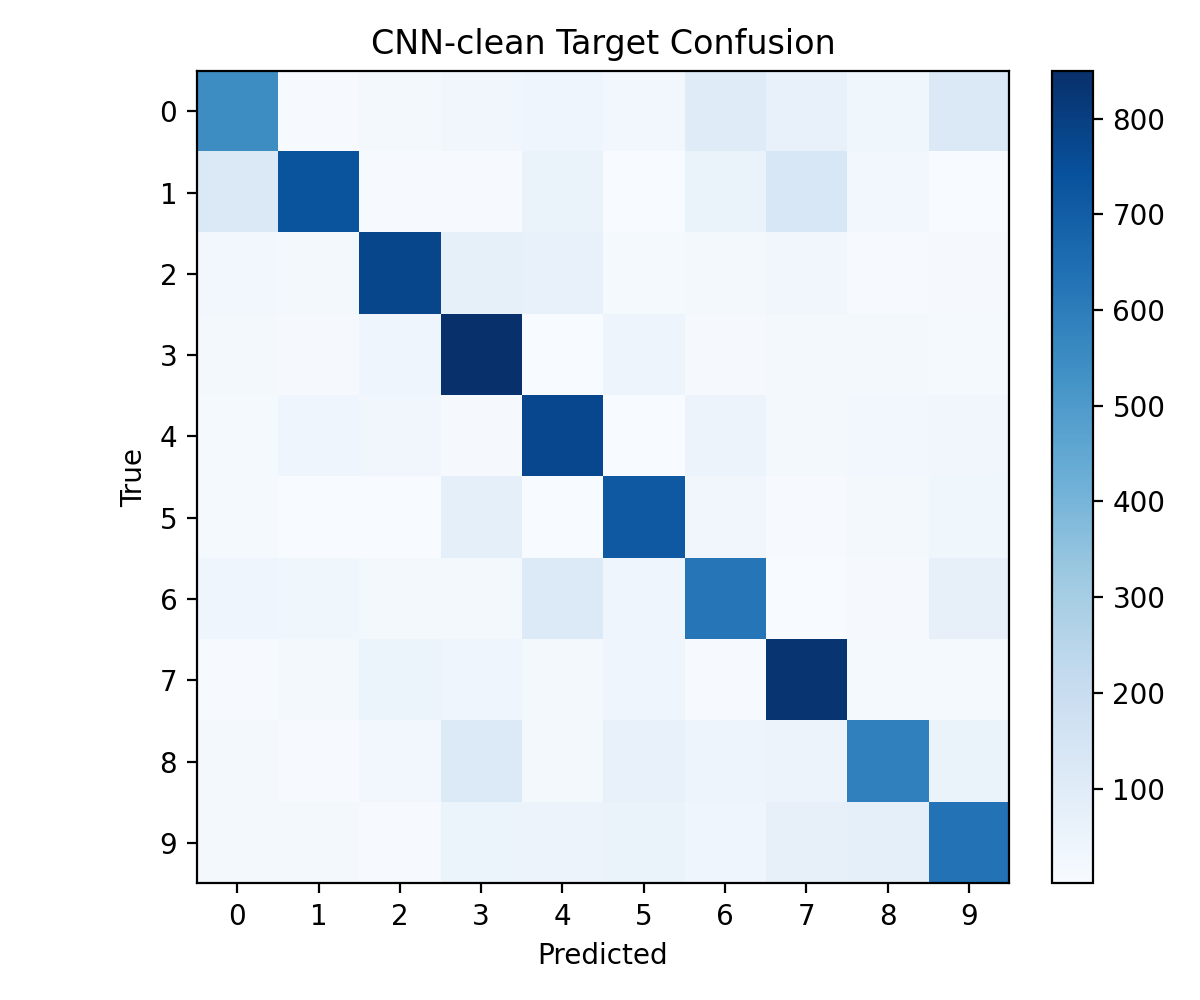
\includegraphics[width=\textwidth]{cnn_clean_target_confusion_matrix.png}
    \caption{\texttt{CNN-clean}}
  \end{subfigure}
  \hfill
  \begin{subfigure}{0.32\textwidth}
    \centering
    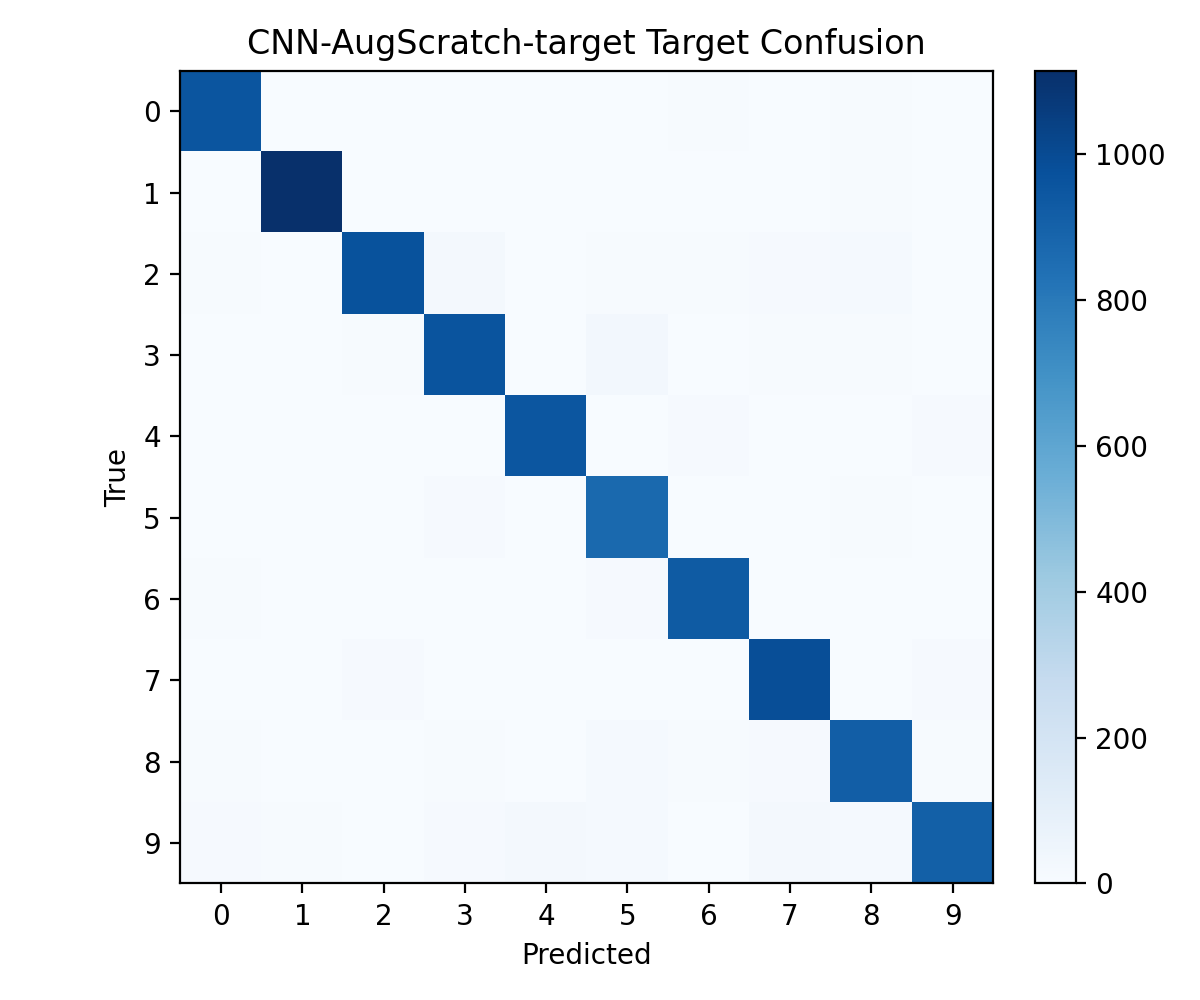
\includegraphics[width=\textwidth]{cnn_augscratch_target_target_confusion_matrix.png}
    \caption{\texttt{CNN-AugScratch-target}}
  \end{subfigure}
  \hfill
  \begin{subfigure}{0.32\textwidth}
    \centering
    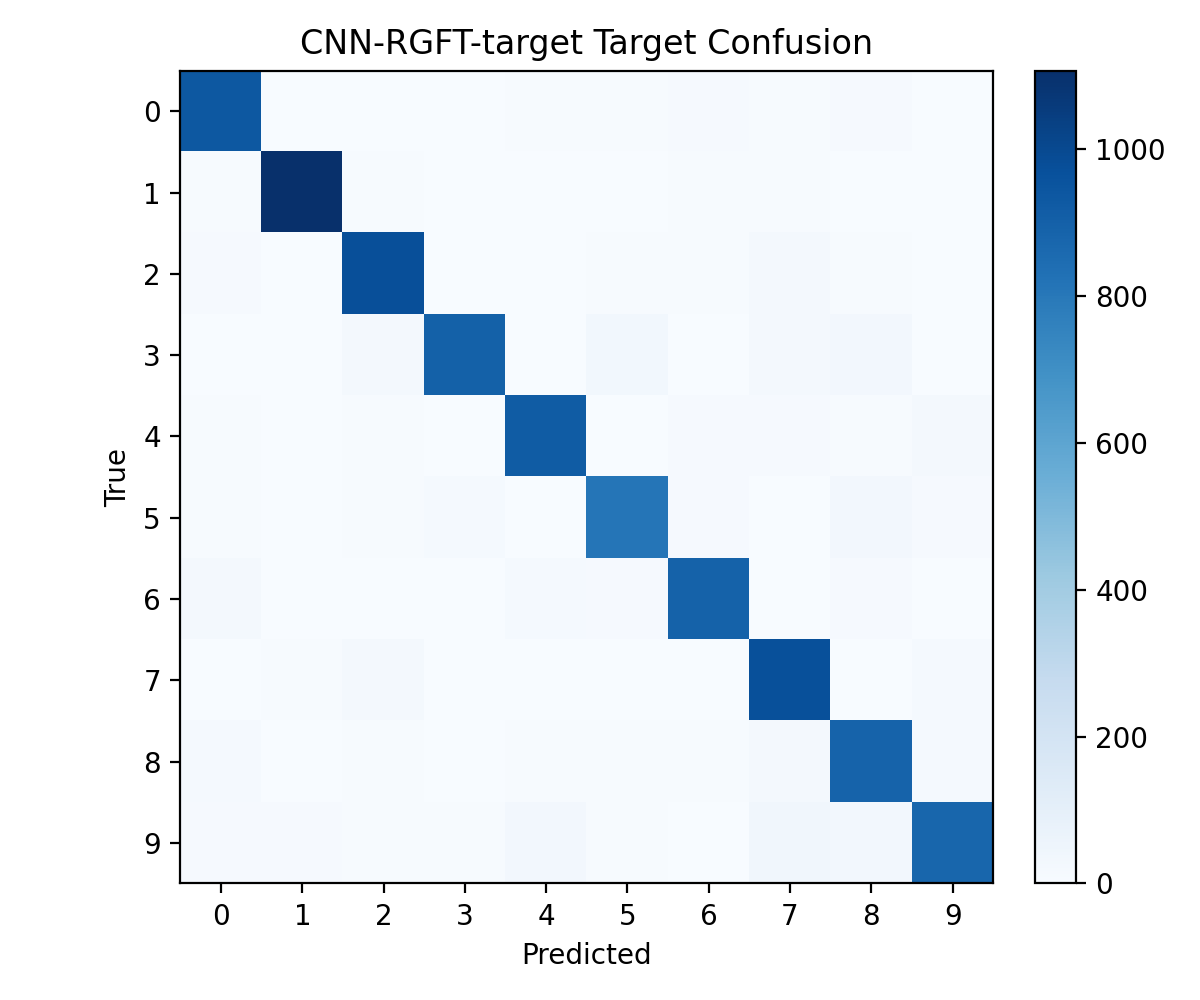
\includegraphics[width=\textwidth]{cnn_rgft_target_target_confusion_matrix.png}
    \caption{\texttt{CNN-RGFT-target}}
  \end{subfigure}
  \caption{Target perturbation 下的 confusion matrices。}
\end{figure}

\begin{figure}[H]
  \centering
  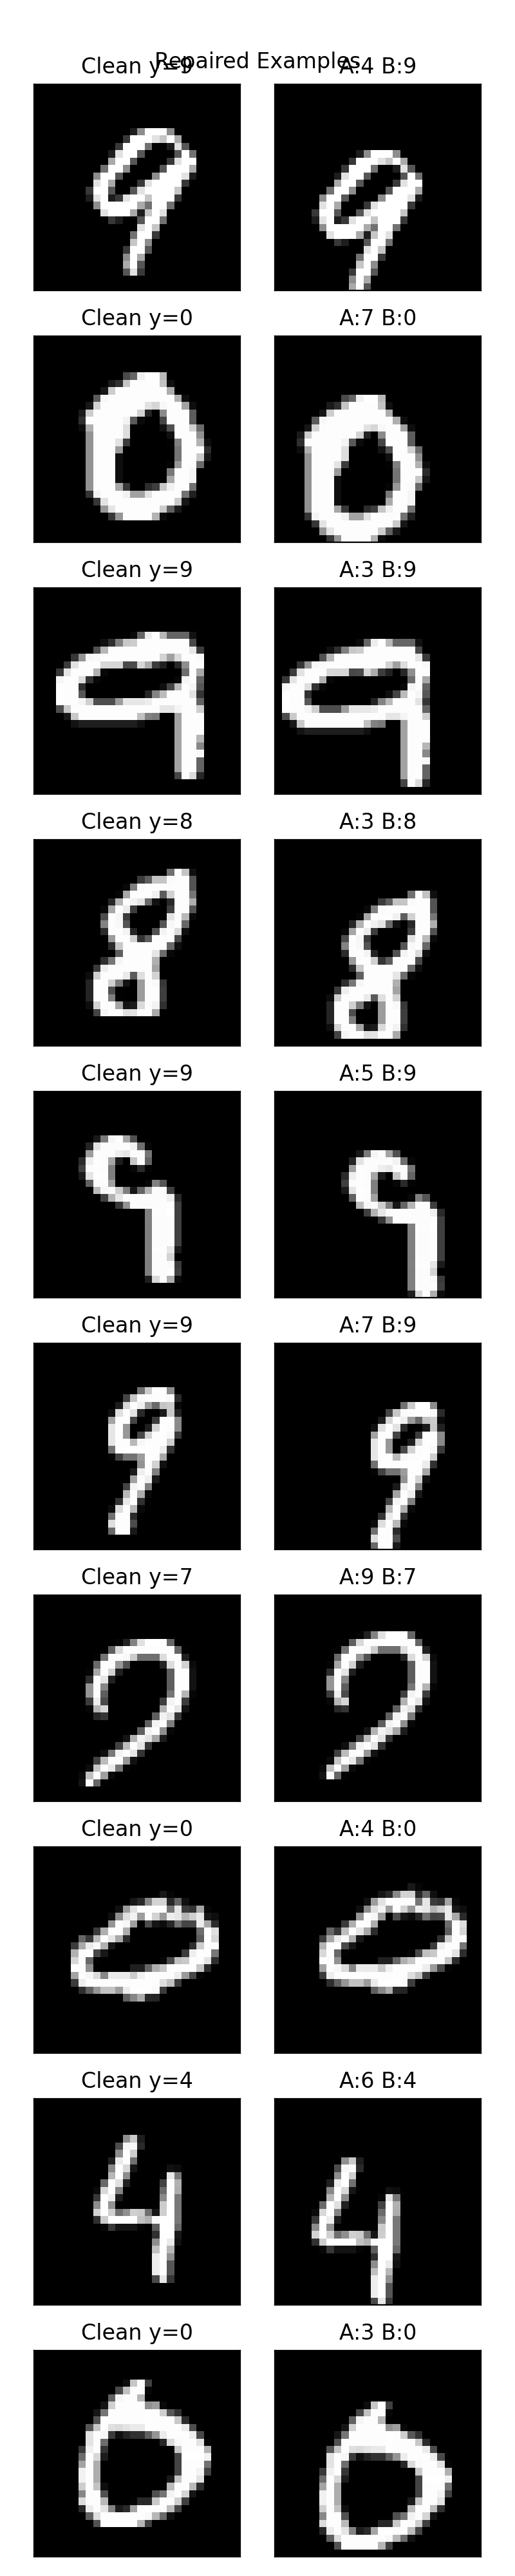
\includegraphics[width=0.60\textwidth,height=0.78\textheight,keepaspectratio,trim=0 0 0 80,clip]{repaired_examples.png}
  \caption{Examples repaired by \texttt{CNN-RGFT-target} under the selected target perturbation.}
\end{figure}

\begin{figure}[H]
  \centering
  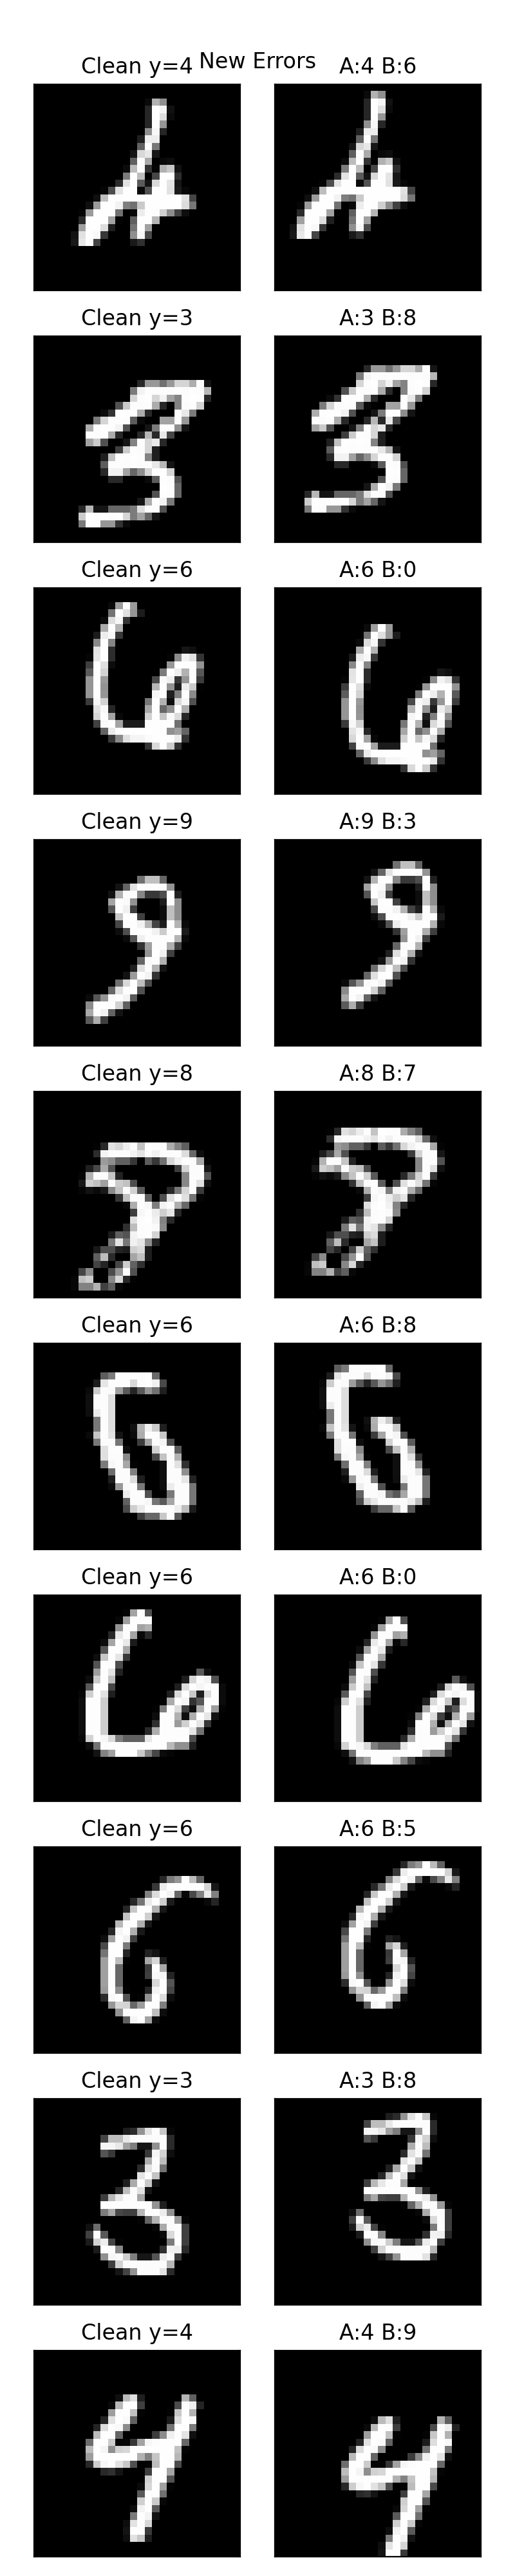
\includegraphics[width=0.60\textwidth,height=0.78\textheight,keepaspectratio,trim=0 0 0 80,clip]{new_errors.png}
  \caption{New errors introduced by \texttt{CNN-RGFT-target} under the selected target perturbation.}
\end{figure}

\section{Main Results and Discussion}

为便于总览，表 \ref{tab:main_results} 汇总了本项目最关键的模型结果。这个总表对应老师要求中的 \texttt{main results table}，而详细曲线、权重可视化、混淆矩阵和 example-level visualization 已经穿插在前述实验部分中。

\begin{table}[H]
  \centering
  \scriptsize
  \caption{本项目主结果总表。}
  \label{tab:main_results}
  \renewcommand{\arraystretch}{1.12}
  \setlength{\tabcolsep}{4pt}
  \begin{tabular}{lcccp{2.8cm}p{4.6cm}}
    \toprule
    模型 & Clean Test & Target Test & Target Drop & 额外代价/预算 & 主要结论 \\
    \midrule
    \texttt{MLP-clean} & 0.9640 & 0.5320 & 0.4320 & clean baseline & 对 selected target 很脆弱。 \\
    \texttt{CNN-clean} & 0.9799 & 0.7069 & 0.2730 & clean baseline & clean accuracy 明显强于 MLP，但 target weakness 仍然存在。 \\
    \texttt{CNN-AugScratch-target} & 0.9815 & 0.9568 & 0.0247 & 30 epochs from scratch & 主线中 target robustness 最强，同时 clean accuracy 也保持最好。 \\
    \texttt{CNN-RGFT-target} & 0.9790 & 0.9266 & 0.0524 & 10 fine-tune epochs & 在已有 clean baseline 的前提下，提供了很强的低边际成本修复。 \\
    \texttt{CNN-RGFT-random10-all} & 0.9765 & 0.8989 & 0.0776 & 50{,}000 sample updates & 小样本 repair 的强 baseline，说明随机覆盖在低预算下很重要。 \\
    \texttt{CNN-RGFT-hard10-all} & 0.9626 & 0.8181 & 0.1445 & 50{,}000 sample updates & hard-only subset 不够稳定，诊断样本不等于最优微调分布。 \\
    \bottomrule
  \end{tabular}
\end{table}

如果直接回答课程要求中的讨论问题，本项目可以得到以下结论。第一，CNN 比 MLP 更适合图像分类，因为它保留局部结构、共享检测器，并能更高效地构建分层特征。第二，CNN 的确同时提升了 validation 和 test accuracy，而且是在更少参数下取得的。第三，我选择的两个 additional directions 是 \texttt{Data Augmentation} 与 \texttt{Robustness Analysis}，因为它们可以组成一条很清楚的因果链：先诊断 weakness，再围绕 weakness 设计 augmentation，而不是随意堆叠变换。

第四，最有信息量的结果并不是某个单一高分，而是“robustness-guided target selection + AugScratch/RGFT comparison + random10 vs hard10 negative finding”这一整条证据链。它一方面证明 target-aware augmentation 的确有效，另一方面也说明 diagnosis-guided hard examples 并不自动等于最好的小预算微调数据。第五，当前仍然困难的样本主要包括两类：一类是本身形状接近、局部笔画容易混淆的数字对，如 $1/7$、$0/9$、$8/3$；另一类是数字主体靠近图像边缘、在平移后关键笔画被截断的样本。这与 \texttt{translation-3} 被选为主要 weakness 是一致的。

\begin{figure}[H]
  \centering
  \begin{subfigure}{0.48\textwidth}
    \centering
    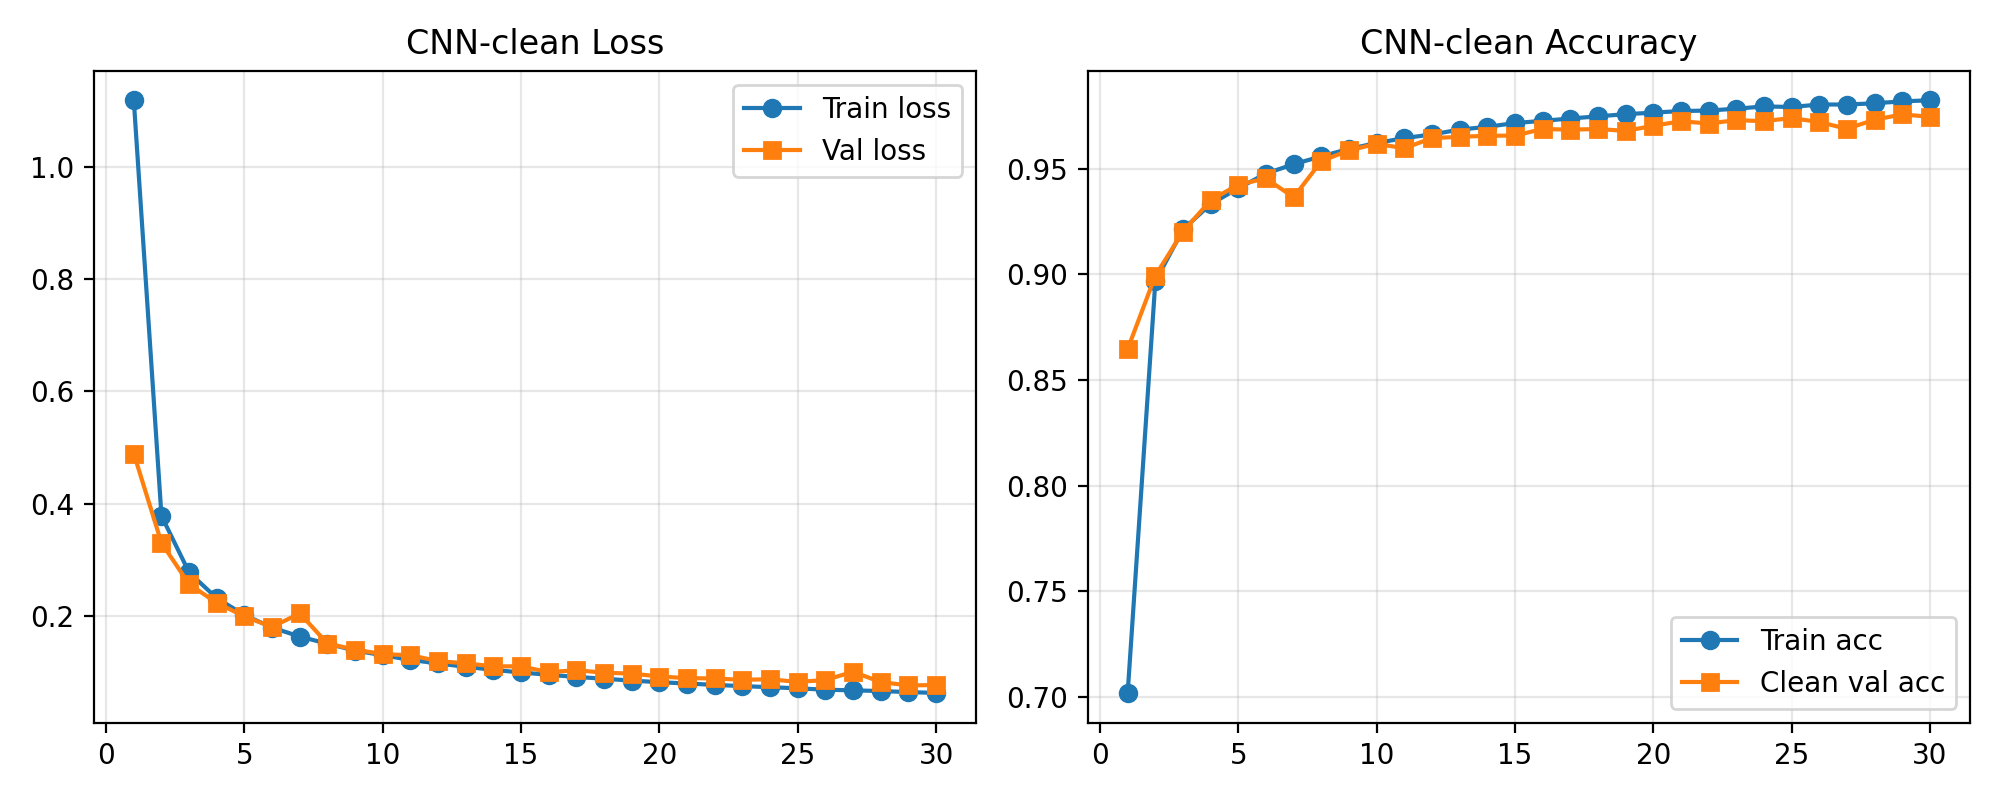
\includegraphics[width=\textwidth]{cnn_learning_curve.png}
    \caption{\texttt{CNN-clean}}
  \end{subfigure}
  \hfill
  \begin{subfigure}{0.48\textwidth}
    \centering
    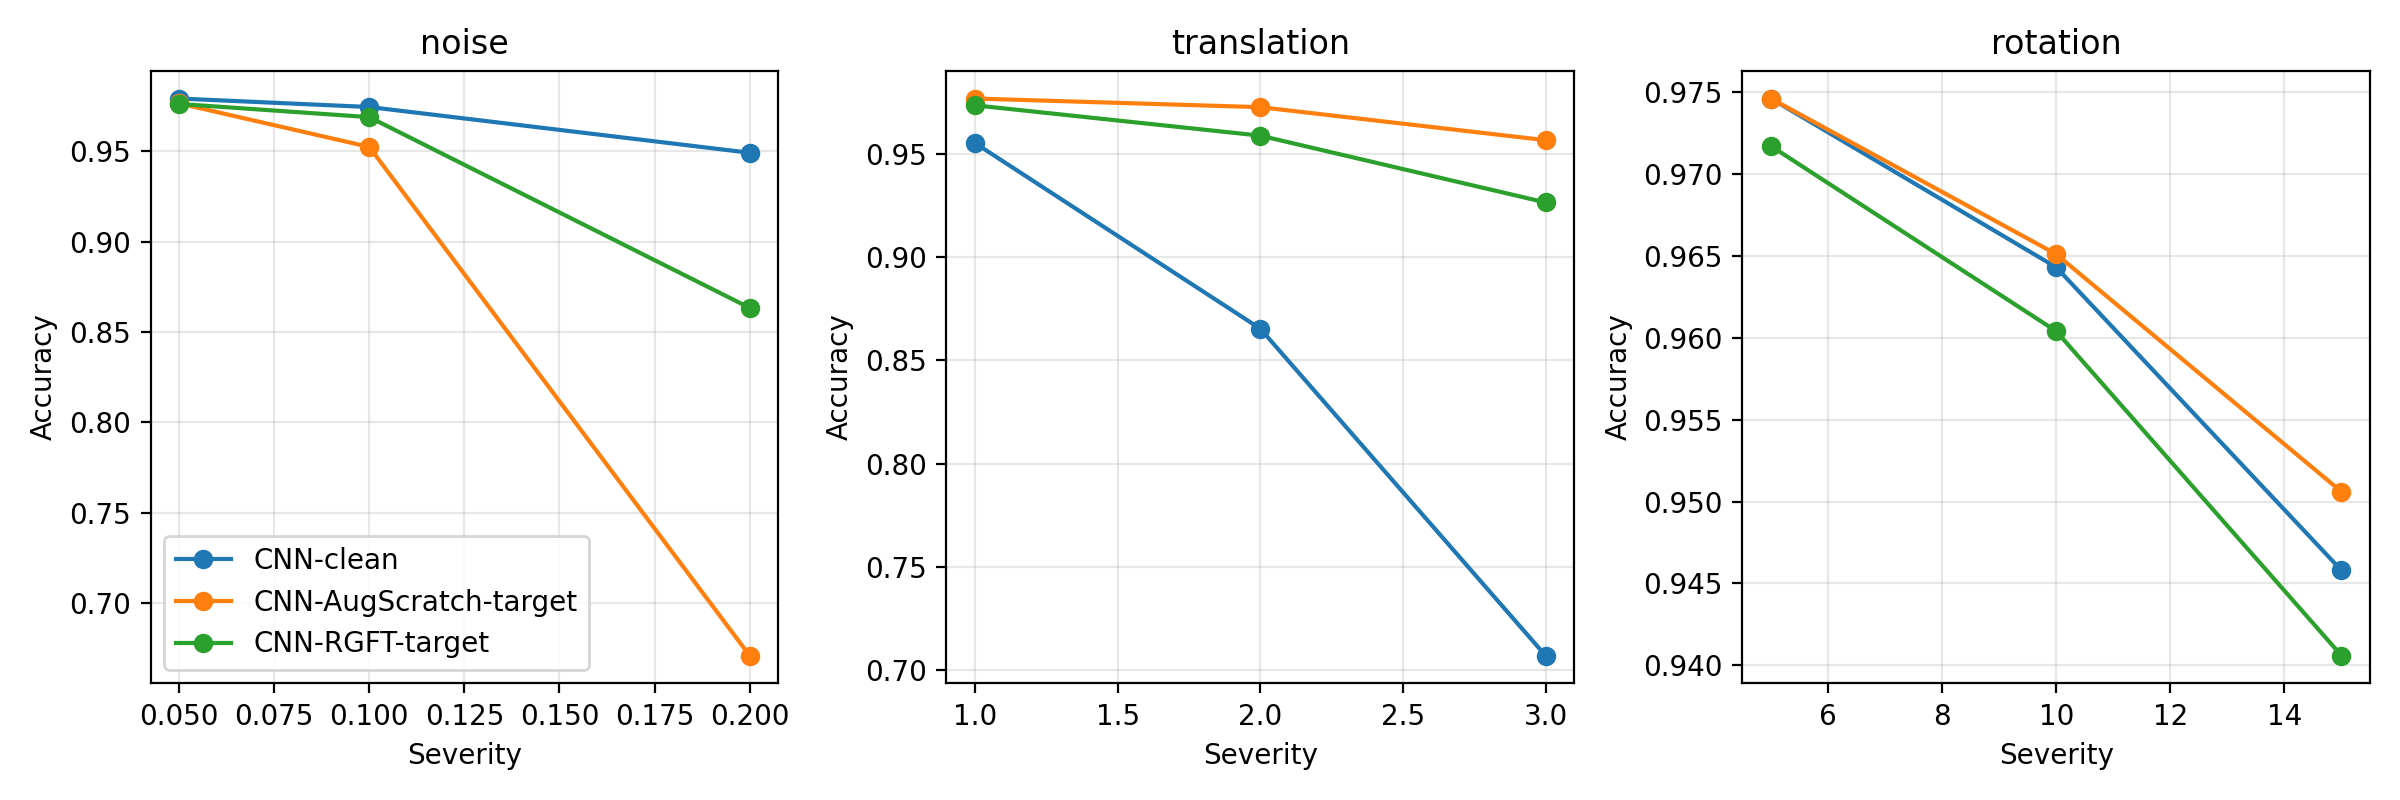
\includegraphics[width=\textwidth]{robustness_curves.png}
    \caption{Main robustness curves}
  \end{subfigure}
  \caption{代表性训练与鲁棒性可视化。}
\end{figure}

\begin{figure}[H]
  \centering
  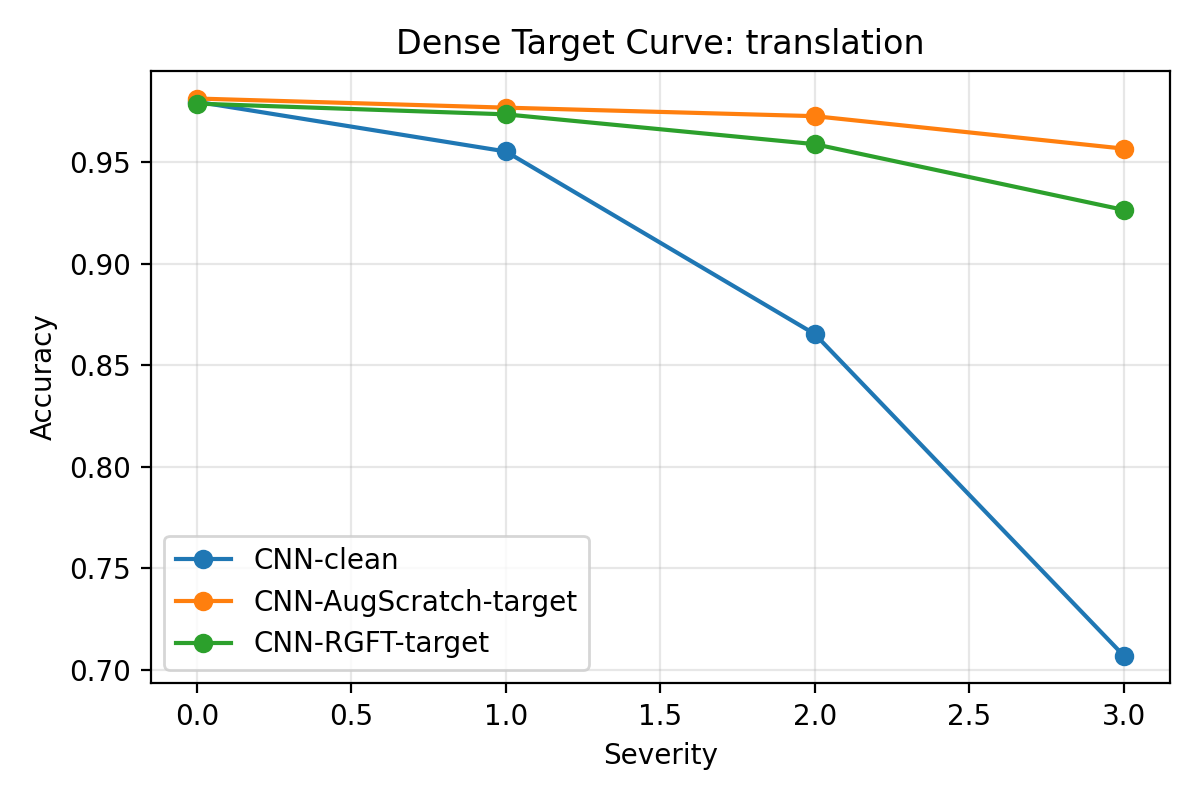
\includegraphics[width=0.72\textwidth]{target_only_dense_curve.png}
  \caption{Accuracy curves under increasing target severity.}
\end{figure}

\section{Conclusion}

整个项目可以概括为三层递进。首先，Part A 证明了从零实现的训练链路是正确的。其次，Part B 表明 CNN 在 clean MNIST 上以更少参数取得了更好的验证与测试性能。最后，Part C 通过 robustness diagnosis 找到了 \texttt{CNN-clean} 的主要 weakness，并证明 target-aware augmentation 可以显著提升该弱点上的鲁棒性，其中从头增强训练效果最强，而 targeted fine-tuning 在已有 clean baseline 的条件下具有很高的边际效率。

更进一步的 extension 给出了一个比“继续刷高分”更有价值的 negative finding：hard examples 对 diagnosis 很有用，但并不一定构成最好的 standalone fine-tuning subset。对于低成本 repair，failure exposure 很重要，但 distribution coverage 同样重要。

\end{document}
